\section{\texorpdfstring{Seiduv switching}{Seiduv switching}}
\vspace{5mm}
\large

\begin{definition}
Nechť V je V.P nad T. Lineární forma je lineární zobrazeni $f:V \to T$. Pak lineární formy tvoří V.P. nad T. Značíme $V^{\ast}$ a je tzv. duální prostor k V.
\end{definition}
\begin{definition}
Nechť $B = \{b_1, b_2, ..., b_n\}$ je báze V, pak $B^{\ast} = \{ f_1, f_2, ..., f_n \}$ je duální báze, pokud formy jsou dáne předpisem:
\[ f_i(b_j)= \twopartdef{1}{i = j}{0}{jinak} \]
\end{definition}
\begin{definition}
Nechť A,B jsou V.P nad T, $dimA = n, dimB = k$. Nechť $\varphi:A \to B$ homomorf. Pak duální homomorf k $\varphi$ je zobrazeni $\varphi^{\ast}: B^{\ast} \to A^{\ast}$ dáne předpisem:
\[ \forall f \in B^{\ast}\  \forall u \in A: (\varphi^{\ast}(f))(u) = f(\varphi(u)) \]
\end{definition}


\begin{theorem}[Matice duálního homomorf(BD)]
Matice duálního homomorf vzhledem k duálním bázím je transponovanou matici k matici primárního homomorf.
\[ \prescript{}{C^{\ast}}{[\varphi^{\ast}]}_{B^{\ast}} = (\prescript{}{B}{[\varphi]}_{C})^T \]
\end{theorem}
\begin{proof}
	Matice zobrazeni lineární formy z prostoru $f:V \to T$ je
	\[ \prescript{}{B}{[f]}_{k} = (f(b_1), f(b_2),...,f(b_n)) \]

	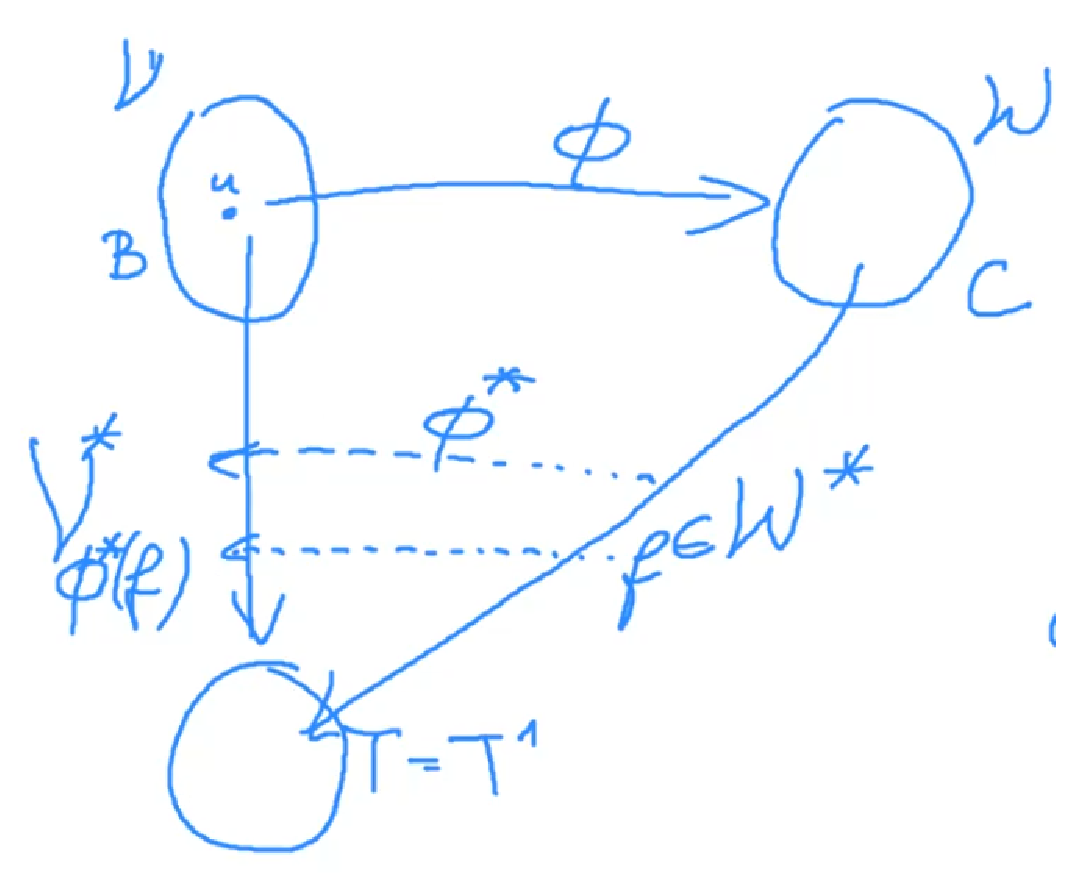
\includegraphics[scale=0.4]{dual_1.eps}

	Máme homomorf $\phi:V \to W$, pak lineární formy $h:W \to T$.

	Duální homomorf $\phi^{\ast}:W^{\ast} \to V^{\ast}$ je definován:
	\[ \phi^{\ast}(f)(u) = f(\phi(u)) \]

	Jelikož lineární formy jsou n-tice, tak $dim(V) = dim(V^{\ast})$.

	Matice $\phi$ je $\prescript{}{B}{[\phi]}_{C} \in T^{k \times n}$.
	Matice $\phi^{\ast}$ je $\prescript{}{C^{\ast}}{[\phi^{\ast}]}_{B^{\ast}} \in T^{n \times k}$.

	Veta říká, ze
	\[ \prescript{}{C^{\ast}}{[\varphi^{\ast}]}_{B^{\ast}} = (\prescript{}{B}{[\varphi]}_{C})^T \]
\end{proof}

\begin{definition}
Faktorprostor: faktorizace dle podprostoru W prostoru V (podgrupa). $V/W$ jsou množiny $\forall u \in V u + W$. Pak i faktorprostor je V.P vůči operacím:
\[ (u + W) + (a + W) = (u + a)W, \lambda \cdot (u + W) = (\lambda \cdot u) + W \]
Platí: $dim(V/W) = dimV - dim W$.
\end{definition}

\begin{theorem}[Izomorfismus faktorprostoru]
	Nechť $V = T^n$ a nechť W je podprostor. Pak
	\[ V/W^{\perp} \sim W^{\ast} \]
\end{theorem}
\begin{proof}
	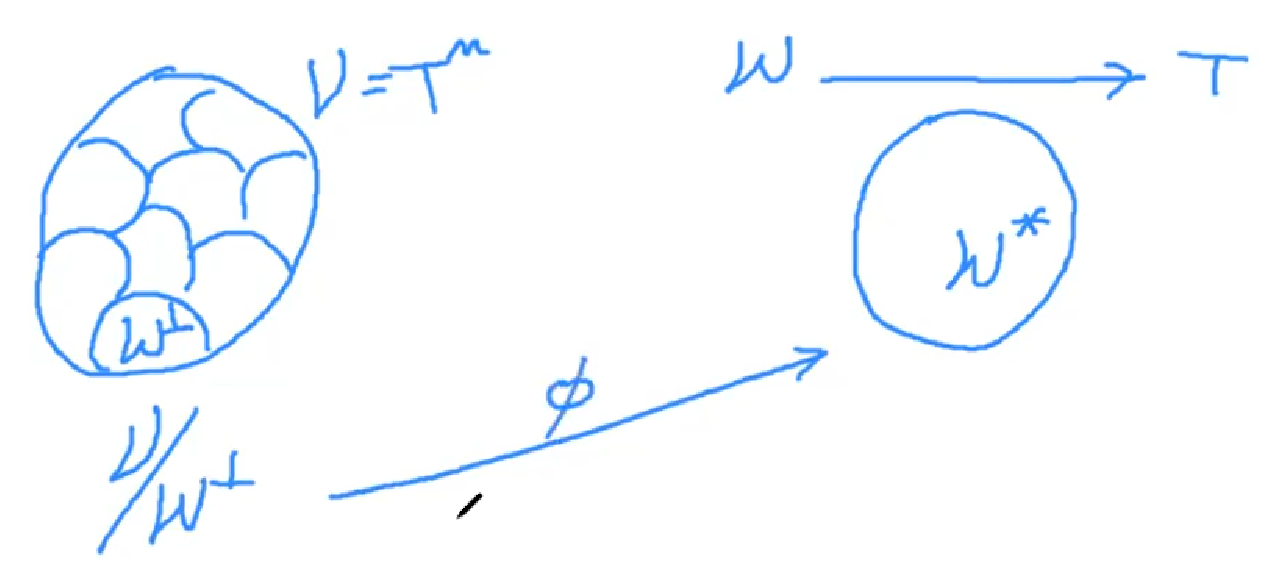
\includegraphics[scale=0.4]{dual_2.eps}

	Pak izomorfizm $\phi$ je definován:
	\[\phi(v + W^{\perp}) = \langle v, \cdot \rangle \]
	Udělali jsme lineární formu z bilineární??

	Pokud dosadíme proměnnou:
	\[\forall x \in W: \phi(v + W^{\perp})(x) = \langle v, x \rangle \]

	Chceme aby $\phi$ bylo korektně definované a splňovalo vlastnosti izomorfuzmu:

	1) korektnost definice \\
	2) lineární zobrazeni \\
	3) proste\\
	4) na

	Důkaz:\\
	1) $a \in v + W^{\perp} \iff a = v + b, b \in W^{\perp}$. Pak
	\[ \langle a, x \rangle = \langle v + b, x \rangle = \langle v, x \rangle + \langle b, x \rangle\]
	Protože $x \in W \Rightarrow \langle b, x \rangle = 0 \Rightarrow \langle v, x \rangle = \langle a, x \rangle $.

	2) Skalární součin je bilineární forma, z toho $\phi$ je lineární zobrazeni.\\
	3) Nechť $\phi(v + W^{\perp}) = 0 \Rightarrow \forall x \in W : \langle v, x \rangle = 0 \Rightarrow v \in W^{\perp} \Rightarrow v + W^{\perp} = \bar{0} + W^{\perp}$.
	Takže v kernelu je pouze $W^{\perp}$.

	4) Nahledneme z dimenzi.
	\[ Im(\phi) \leq W^{\ast} \land dim(Im(\phi)) = dim (V/W^{\perp}) \]
	Rovnost dimenzi platí protože zobrazeni je prosté.
	\[ dim(Im(\phi)) = dim(V) - dim(W^{\perp}) = dim(V) - (dim(V) - dim(W)) = dim(W) = dim(W^{\ast}) \]

	Z LA $Im(\phi)$ je vnořený podprostor stejné dimenzi jako nadprostor $\Rightarrow$ jsou stejné.

\end{proof}

\begin{theorem}[Burnsidovo lemma(BD)]
\end{theorem}

\begin{lemma}
Nechť grupa $G$ provádí akci na množině $M$, grupa $H$ na $N$. Nechť $\varphi:M \to N$ bijekce.
	\[ if g \in G, h \in H, \forall m \in M: h\varphi(m) = \varphi(gm) \Rightarrow |G_{g}| = |H_{h}| \]

	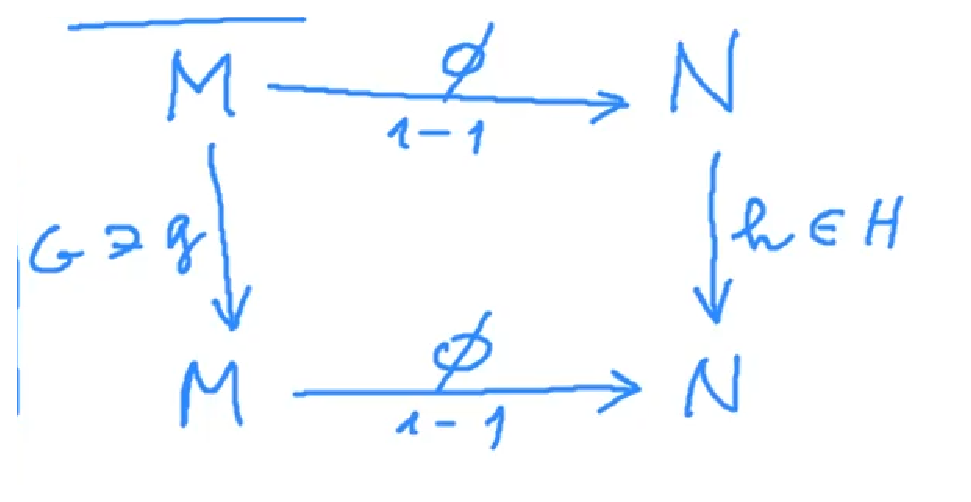
\includegraphics[scale=0.4]{group_lemma.eps}
\end{lemma}
\begin{proof}
Prvky v $M_g$ jsou $gm = m$. Prvky v $N_h$ jsou $hn = n$. Kvůli bijekci $n$ lze jednoznačně vyjádřit jako:
\[ n = \varphi(m) = \varphi(\varphi^{-1}(n)) \]
Pak
\[ h\varphi(m) = \varphi(m) \]
Diagram komutuje
\[ \varphi(gm) = \varphi(m) \]
$\varphi$ je bijekce, takže prosté $\Rightarrow gm = m$. Dohromady \# $hn = n$ je totéž jako \# $gm = m$.
\end{proof}

\begin{definition}
Seiduv switching vymění všechny hrany a nehrany výcházející z $u \in V$. Ostatní vrcholy a hrany beze změn. Grafy $G \sim G' \iff G'$ lze získat z $G$ postupným přepinaním vrcholu.
\end{definition}

\begin{note}
	\[ G \sim G' \iff \exists A \subseteq V(G): G' = S(G,A) \]
	kde $S(G,A)$ je switch cele podmnožiny. Hrany mezi A a zbytkem se prohodí.
\end{note}

\begin{note}
	Dva grafy na stejné množině vrcholu jsou Seidelovsky ekvivalentní $\iff$ jsou ve stejné třídě faktorizace $V_{K_V}/ \beta_{K_V}$.
	Proto je tříd ekvivalence tolik, kolik je Eulerovských grafu na dáne množině vrcholu.
\end{note}

\begin{theorem}[Pocet neiz trid Seide switching]
Počet neizomorfních tříd ekvivalence při Seidelově switchingu na $n$ vrcholech je roven počtu Eulerovských grafů na $n$ vrcholech.
\end{theorem}
\begin{proof}
Pro lichá $n$, označme
\[ \{ A = \{ u | deg_G(u) \equiv 1 \mod2 \}, |A| \equiv 0 \mod2\ \]

	Uděláme switch množiny A: $(G,A)$. Vezmeme vrchol $u \in V\setminus A$
	Pak $deg_G(u) = a + b$, kde $a$ je počet hran mimo $A$, $b$ je počet hran vedoucích do $A$.

	Po switchu:
	\[ deg_{S(G,A)}(u) = a + |A| - b = deg_G(u) - 2b - |A| \equiv 0 \mod2 \]

	Vezmeme vrchol $u \in A, deg_G(u) = c + d$, kde $c$ jsou hrany v A, $d$ hrany mimo A.

	Po switchu:
	\[ deg_{S(G,A)}(u) = c + |V \setminus A| - d = c + d - 2d + |V| - |A|\]
	Kde $(c + d)$ je liché, $|V|$ je liché, $|A|$ je sude. Dohromady sude.

	Takže kazdy graf lze přeswitchovat na Eulerovský graf. Přeswitcheni Eulerovského grafu se změní na neeulerovský. V každém switching třídě je 1 Eulerovský graf.

	Pro $n$ sude. Nechť $\nu$. je V.P. všech grafu na dáne množině vrcholu, $B$ je prostor elementárních řezu na uplném grafu, $\xi$ prostor Eulerovských grafu.
	\[ \beta = \xi^{\perp} \Rightarrow \xi^{\ast} \simeq \nu/B \]

	Prvky $\nu/B$ jsou právě třídy ekvivalence dle Seidelovem switchingu. Chceme zjistit počet orbit akci grupy $S(V)$.

	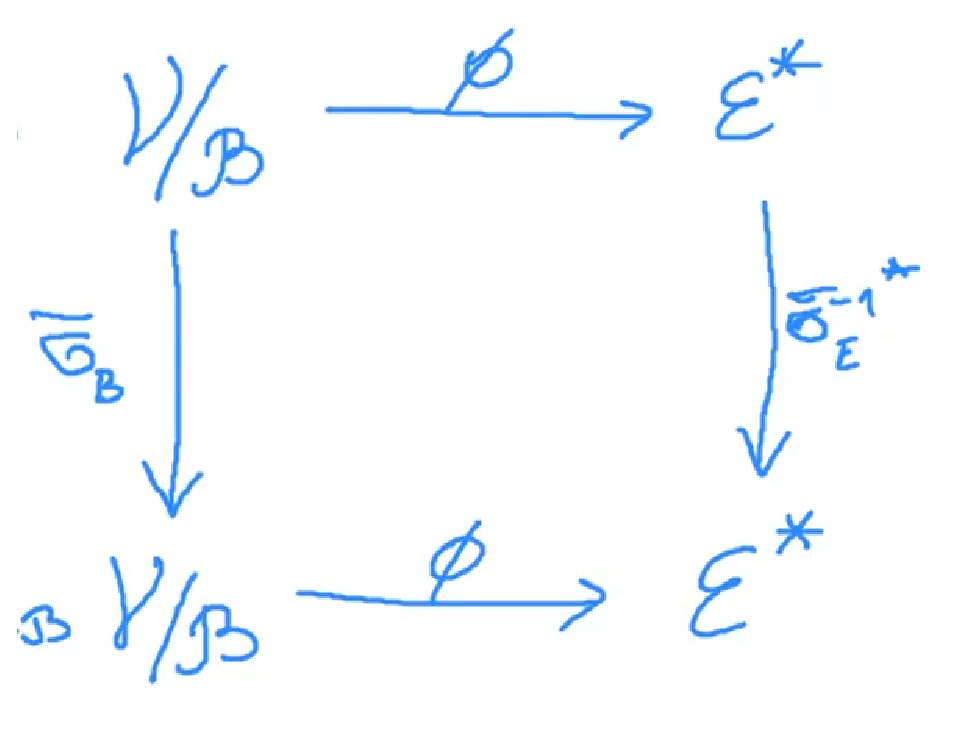
\includegraphics[scale=0.4]{seide_1.eps}
	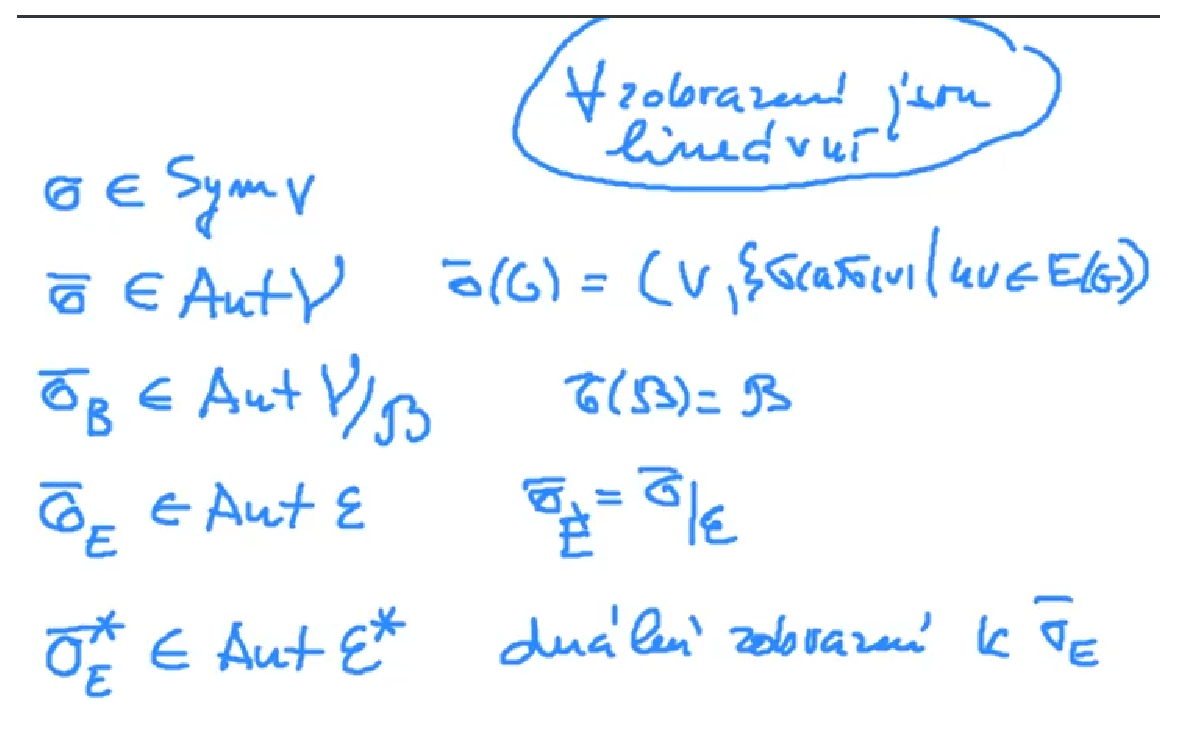
\includegraphics[scale=0.4]{seide_2.eps}

	Tvrdíme ze diagram komutuje. Nechť $G \in \nu$
	\[ \bar{\sigma}_B(G + B) \to \sigma(G) + B, \phi(\sigma(G) + B) \to \langle \bar{\sigma}(G), \cdot \rangle \in \xi^{\ast} \]
	\[ \phi(G + B) \to \langle G, \cdot \rangle \in \xi^{\ast}, (\bar{\sigma}^{-1})^{\ast}(\langle G, \cdot \rangle) \]

	Tvrdíme ze poslední prvky ve dvou řádcích jsou stejné.
	\[ \forall X \in \xi: \langle \bar{\sigma}(G)(X) \rangle = (\bar{\sigma}^{-1})^{\ast}(\langle G, \cdot \rangle) = \langle G, (\bar{\sigma}^{-1})(G) \rangle \]
	Levá část
	\[ \langle \bar{\sigma}(G)(X) \rangle = |\{ e | e \in E(\bar{\sigma} \cap E(X) \} \]
	Pravá část
	\[ \langle G, (\bar{\sigma}^{-1})(G) \rangle = |\{ e | e \in E(G) \cap (\bar{\sigma}^{-1})(X) \} \]
	Z toho diagram komutuje.

	Pak dle Burnsidova lemmatu: \# orbit $\nu/B$ při akci $S(\nu) = \frac{1}{n!} \sum |(\nu/B)_{\sigma}|$.

	Taky \# orbit $\xi^{\ast}$ při akci $S(V) = \frac{1}{n!} \sum |(\xi^{\ast})_{\sigma}| = \frac{1}{n!} \sum |(\nu/B)_{\sigma^{-1}}|$.
%todo
	Zbývá dokázat, ze \# orbit je stejný i pro $\xi$ místo $\xi^{\ast}$.

\end{proof}
